\chapter{Application to a dynamically twisted flux tube}

\label{chp:kink_instability_straight}

\graphicspath{{images/kink_instability_straight/}}

\section{Introduction}

In chapter~\ref{chp:kink_instability} the dynamics in a magnetic flux rope which is already linearly unstable to the helical kink instability were investigated. An alternative way to excite the kink instability is to start with an initially straight field and apply twisting motions at the boundaries to create a twisted flux rope which eventually becomes unstable to the kink instability. In addition, a fluting instability is found to be excited prior to the development of the kink instability. To our knowledge, this is the first time a fluting instability in coronal conditions has been studied through 3D numerical simulations. 

The fluting instability arises in magnetised plasmas where the plasma pressure gradient is directed in the same direction as the field line curvature, that is the pressure and magnetic tension forces compete. This is similar to the competition between pressure and gravitational forces which gives rise to the Rayleigh-Taylor instability (RTI). In a twisted flux tube like a coronal loop, the tube may be unstable to fluting when the pressure decreases outwards from the core. The ideal fluting instability is simply an ideal interchange instability in a cylindrical flux tube. \todo{ref to later plot of field lines + pressure contours}

In the study of coronal loops, the main focus has been the ideal kink instability (see chapter~\ref{chp:kink_instability}). We do not know of any coronal studies of the fluting instability specifically in coronal loops. In other solar contexts, we find interchange instabilities in the form of ballooning modes in arcades~\cite{hoodBallooningInstabilitiesSolar1986}, as the instability which forms tubes of specific size in the photosphere~\cite{bunteInterchangeInstabilitySolar1993} and in the buoyancy of flux tubes~\cite{schuesslerInterchangeInstabilitySmall1984}. The instability is more commonly studied in fusion contexts.

While the stability of the ideal fluting instability has been studied extensively in fusion research~\cite{mikhailovskiiInstabilitiesConfinedPlasma1998,zhengAdvancedTokamakStability2015,wessonHydromagneticStabilityTokamaks1978}, the focus is generally on understanding how a particular plasma device may be stabilised to the instability in particular geometries such as that of the mirror machine~\cite{jungwirthTheoryFluteInstability1965} or in toroidal geometries such as the tokomak~\cite{shafranovFluteInstabilityCurrentcarrying1968}. The resistive interchange instability (the resistive form of the fluting instability) can be excited even when the ideal fluting instability is stabilised. As a result, this has been given significantly more attention~\cite{johnsonResistiveInterchangesNegativeV1967,correa-restrepoResistiveBallooningModes1983}.

\subsection{Introduction to fluting stability}

In general, the stability of a cylindrical twisted magnetic flux tube is analysed using perturbations of the form
\begin{equation}
  \label{eq:kink_perturbation}
\xi(r, \theta, z) = \xi(r) e^{i(m\theta + kz)},
\end{equation}
where $m$ and $k$ are the wavenumbers in the $\theta$ and $k$ directions, respectively. The helical kink instability occurs for perturbations where $m=1, k\ne0$ and is the only instability of this form which is a body instability, that is it moves the entire body of the flux tube. Perturbations where $m>1$ are fluting or interchange instabilities.

When the magnetic field is sheared, as in a twisted magnetic flux tube, an interchange instability (such as the fluting instability) is confined to a surface where the peaks and troughs follow the shear of the field. That is, a surface where the perturbation wavevector $(0, m/r, k)$ is perpendicular to the direction of the field. In an axisymmetric, twisted flux tube the resonant surface is located at a radius $r$ given by
\begin{equation}
  \label{eq:resonant_surface}
\frac{m}{r} B_{\theta}(r) + kB_z(r) \approx 0.
\end{equation}
In contrast to kink instabilities, fluting instabilities are surface instabilities.

The stability of a cylindrical flux tube to perturbations of the form~\ref{eq:kink_perturbation} is given by the classical Suydam's criterion
\begin{equation}
  \label{eq:suydams_criterion}
\frac{B_z^2 S^2}{4} + 2 r p' > 0,
\end{equation}
where $S = r q'/q$ is a measure of the shear and $q = 2\pi r B_z / L B_{\theta}$ is the safety factor~\cite{mikhailovskiiInstabilitiesConfinedPlasma1998}. Where~\ref{eq:suydams_criterion} is unsatisfied, the flux tube may be unstable to perturbations of the form~\ref{eq:kink_perturbation}. When $m>1$, the perturbations remain local to resonant surfaces given by~\ref{eq:resonant_surface}.

When the criterion is satisfied and the flux tube is linearly stable, it may still be unstable to non-local perturbations, where the shear and pressure are low enough that interchange perturbations do not need to satisfy~\ref{eq:resonant_surface}. Additionally, the inclusion of resistivity generally reduces the stabilising effect of the shear, permitting growth of a resistive interchange mode, albeit at a lower rate than that in the ideal case. It will be found that the ideal linear analysis is sufficient for understanding the fluting instabilities investigated in this chapter since the flux tubes investigated here adequately fail the criterion~\ref{eq:suydams_criterion}.

The linear growth rate of the ideal fluting instability $\gamma$ can be found via a stability analysis analogous to that of the Rayleigh-Taylor instability (see~\cite{goldstonIntroductionPlasmaPhysics2020}) and is given by
\begin{equation}
  \label{eq:fluting_growth_rate}
\gamma^2 = \frac{2|\nabla p|}{\rho R_c},
\end{equation}
where $R_c$ is the radius of curvature of the magnetic field. This equation only applies when the pressure gradient and radius of curvature vector are in the same direction, that is the plasma is constrained by a concave magnetic field such that the pressure forces and magnetic tension forces are in competition. In a cylindrical, twisted flux tube, the field is always concave towards the central axis of the tube, so any inwardly directed plasma gradient is unstable to fluting.

Throughout this chapter, the twisted flux tube generated by the drivers has a pressure profile which is axisymmetric and approximately independent of $z$ away from the boundaries at $z=\pm2$, hence we may write $\nabla p = d p/ dr$. Similarly, away from the boundaries, we find the magnetic field to have a negligible $r$ component and little dependence on $\theta$ and $z$, allowing the field to be approximated as $\vec{B} = (0, B_{\theta}(r), B_z(r))$, in cylindrical coordinates $(r, \theta, z)$. For a twisted field of this form, the radius of curvature is given by 
\begin{equation}
  \label{eq:radius_of_curvature}
  R_c = \frac{1}{|(\vec{b}\cdot\nabla) \vec{b}|} = \frac{r}{b_{\theta}^2},
\end{equation}
where $\vec{b} = \vec{B}/|\vec{B}|$ is the unit vector in the direction of the magnetic field and $b_{\theta}$ is the component of $\vec{b}$ in the azimuthal direction. These approximations allows us to write the growth rate as
\begin{equation}
  \label{eq:fluting_growth_rate2}
\gamma_{ideal}^2 = \frac{-2p'}{\rho R_c},
\end{equation}
where $p'$ refers to the derivative of $p$ with respect to $r$.

In contrast to the precise form of the equilibrium state and perturbation studied in chapter~\ref{chp:kink_instability}, this is an experiment where a system is driven and instabilities occur naturally as a result of noise providing a random perturbation. As a result of the driving, the flux tube is not in static equilibrium. Consequently, the results of the linear stability analysis summarised previously are useful as a guide and approximate comparison, but should not be considered as an appropriate prediction of growth rates or overall stability.

\section{Methods}

\subsection{Numerical setup}

To investigate a simple, null-free topology, we start with a straight, uniform field
\begin{equation}
\vec{B} = (0, 0, 1)^{\text{T}},
\end{equation}
in a cube of dimension $[-2,2]^3$. The velocity is set everywhere to $\vec{u} = \vec{0}$, the density to $\rho = 1$, the internal energy to $\varepsilon = 8.67\times 10^{-4}$ (corresponding to a temperature of $10^6$K). At the boundaries the magnetic field, density, and energy are fixed to their initial values and the velocity zero except at the upper and lower boundary where the twisting driver, described below, is prescribed. The spatial derivatives of these variables are also set to zero at the boundaries. The resolution is $512$ grid points per dimension, comparable to the highest resolution kink instability studies of~\cite{hoodCoronalHeatingMagnetic2009} or medium resolution studies of~\cite{barefordShockHeatingNumerical2015}. The switching parameter was set to $a_0 = 150$, a value which ensures the viscosity is anisotropic throughout the entire domain. 

\begin{figure}[t]
  \centering
  \begin{subfigure}{.49\textwidth}
  \centering
  \includegraphics[width=1.0\linewidth]{u_r.pdf}
  \caption{Radial dependence of driver}
  \label{fig:kink_radial_driver}
  \end{subfigure}
  \begin{subfigure}{.49\textwidth}
  \centering
  \includegraphics[width=1.0\linewidth]{u_t.pdf}
  \caption{Acceleration of driver}
  \label{fig:kink_driver_accel}
  \end{subfigure}
  
  \caption{Driver velocity radial profile $u(r)$ and acceleration profile $u(t)$.}
  \label{fig:kink_driver}
\end{figure}

The flux rope is formed by prescribing a slowly accelerating, rotating flow at the upper $z$-boundary as
\begin{equation}
  \label{eq:null_twisting_profile}
  \vec{u} = u_0 u_r(r) u_t(t) (-y, x),
\end{equation}
where $u_r(r)$ describes the radial profile of the twisting motion in terms of the radius $r^2 = x^2 + y^2$,
\begin{equation}
  \label{eq:radial_twisting_function}
  u_r(r) = u_{r0}(1 + \tanh(1 - r_d r^2)),
\end{equation}
where $r_d$ controls the radial extent of the driver, $u_{r0}$ is a normalising factor, and $u_t(t)$ describes the imposed acceleration of the twisting motion,
\begin{equation}
  \label{eq:ramping_up_function}
  u_t(t) = \tanh^2(t/t_r),
\end{equation}
where the parameter $t_r$ controls the time taken to reach the final driver velocity $u_0$. The functions $u(r)$ and $u(t)$ are plotted in figure~\ref{fig:kink_driver}. At the lower boundary, the flow is in the opposite direction. This driver, the same as is used in the chapter~\ref{chp:null_point_khi}, allows the driver to be accelerated slowly enough that disruptive shocks and fast waves are not generated. The driver does still generate small torsional Alfv\'en waves. The driver velocity is set to $u_0 = 0.15$, the normalising factor is $u_{r0} = 2.08$, and setting $r_d = 5$ corresponds to a driver constrained to $r<1$ and with a peak velocity at $r\approx 0.38$. The ramping time is set to $t_r = 2$, resulting in an acceleration from $0$ to $u_0$ over approximately $5$ Alfv\'en times. 

These driver parameters correspond to a peak rotational period of $T_R = 15.92$, the length of time taken for one full turn to be injected by a single driver. Both drivers result in twist being added at a rate of $2\pi$ every $7.96$ Alfv\'en times. The twist profile develops in such a way that it is qualitatively similar to that studied in chapter\ref{chp:kink_instability} by $t\approx 20$, however the length of the flux tubes differs significantly. 

This configuration produces a $z$-directed tube of increasingly twisted magnetic field that eventually becomes unstable to both the fluting instability and the helical kink instability. The perturbation for both instabilities develops naturally from numerical noise. Although the setup is similar to that of a twisted coronal loop, including the resulting kink instability, it is not intended to be a realistic simulation of an erupting loop. Similarly, although use is made of the results of a linear stability analysis, the twisted tube which develops in the course of the simulation is not in MHD equilibrium and the stability analysis results have limited applicability as a result.

Although the switching model is used in these experiments, the switching parameter is set to $a_0 = 150$ which reduces the model to purely parallel anisotropic viscosity everywhere, since there are no null points at any point during the simulations. 

\section{Results}

The overall development of both instabilities are broadly similar for the two values of resistivity so we initially focus on the development of the $\eta=10^{-4}$ case, comparing the results of the two viscosity models. Then the differences between the results for the two values of resistivity are summarised without a full exploration of the qualitatively similar $\eta=10^{-3}$ results.

In all cases, the initial reaction to the twisting at the upper and lower boundaries is two torsional Alfv\'en waves which travel along the tube from the upper and lower boundaries to the opposite boundary. The interaction between these waves produces an oscillating pattern in the kinetic energy with a period of approximately $4$, equal to the time taken for an Alfv\'en wave to travel the entire length of the domain (visible early in figure~\ref{fig:kink_ke-4}). As the field is twisted, currents form due to the local shear in the magnetic field and heat the plasma locally through Ohmic heating. Due to the radial form of the driver, the current is greatest at the axis of the tube, then decreases radially outwards, up to a shell of increased current due to the shear between the field in the driven region and the straight, outer field. The gradient in the current produces a gradient in the pressure, with the highest pressure found at the axis of the tube. This provides the inwardly-directed pressure gradient which competes with the twisted magnetic field and is unstable to the fluting instability. The continued driving at the boundaries eventually injects enough twist that the tube also becomes unstable to the kink instability which develops linearly alongside the fluting instability and then erupts during its nonlinear phase, dominating the dynamics and disrupting the fluting instability. The development of the two instabilities is strongly affected by the value of $\eta$ and the viscosity model used.

\subsection{Development where $\eta=10^{-4}$}

\begin{figure}[t]
  \centering
    %\begin{subfigure}{0.32\textwidth}
      %\includegraphics[width=\linewidth]{iso-4_pressure_13.pdf}
      %\caption{iso; $t=26$}
      %\label{fig:iso-4_pressure_13}
    %\end{subfigure}
    %\hfill
    %\begin{subfigure}{0.32\textwidth}
      %\includegraphics[width=\linewidth]{iso-4_pressure_14.pdf}
      %\caption{iso; $t=28$}
      %\label{fig:iso-4_pressure_14}
    %\end{subfigure}
    %\hfill
    %\begin{subfigure}{0.32\textwidth}
      %\includegraphics[width=\linewidth]{iso-4_pressure_15.pdf}
      %\caption{iso; $t=30$}
      %\label{fig:iso-4_pressure_15}
    %\end{subfigure}
    %\hfill
    \begin{subfigure}{0.32\textwidth}
      \includegraphics[width=\linewidth]{swi-4_pressure_13.pdf}
      \caption{$t=26$}
      \label{fig:swi-4_pressure_13}
    \end{subfigure}
    \hfill
    \begin{subfigure}{0.32\textwidth}
      \includegraphics[width=\linewidth]{swi-4_pressure_14.pdf}
      \caption{$t=28$}
      \label{fig:swi-4_pressure_14}
    \end{subfigure}
    \hfill
    \begin{subfigure}{0.32\textwidth}
      \includegraphics[width=\linewidth]{swi-4_pressure_15.pdf}
      \caption{$t=30$}
      \label{fig:swi-4_pressure_15}
    \end{subfigure}
\caption{Pressure profiles during the development of the fluting and kink instabilities. Shown are slices of pressure through $z=0$ where $\eta = 10^{-4}$ and the viscosity model is switching. The development in the isotropic case is similar.}
\label{fig:kink_pressure_slices-4}%
\end{figure}

Figure~\ref{fig:kink_pressure_slices-4} shows the pressure profile through $z=0$ where $\eta=10^{-4}$ and the viscosity model is switching for times $t=26$, $28$ and $30$. The tube becomes notably unstable to the $m=4$ fluting instability at $t=26$, when the plasma begins to bulge out diagonally (figure~\ref{fig:swi-4_pressure_13}). As the bulges move radially outwards into lower pressure regions they expand and accelerate, resulting in the entire pressure structure appearing clover-shaped (figure~\ref{fig:swi-4_pressure_14}). The instability does not strongly affect the tube near the axis, allowing the kink instability to develop simultaneously throughout the growth of the fluting instability. By $t=30$ the kink instability has disrupted the fluting instability and is developing nonlinearly (figure~\ref{fig:swi-4_pressure_15}). As is typical of nonlinear kink development, the tube continues to release its stored potential energy as kinetic energy and heat and the contained plasma becomes highly mixed. In the unseen isotropic case, the fluting instability is present but strongly damped, and the kink instability quickly dominates the dynamics.

\begin{figure}[t]
  \centering
    \begin{subfigure}{0.49\textwidth}
      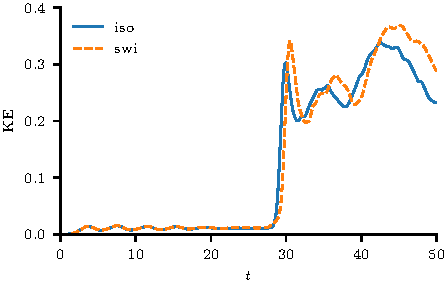
\includegraphics[width=\linewidth]{kinetic_energy-4.pdf}
      \caption{Kinetic Energy}
      \label{fig:kink_ke-4}
    \end{subfigure}
    \hfill
    \begin{subfigure}{0.49\textwidth}
      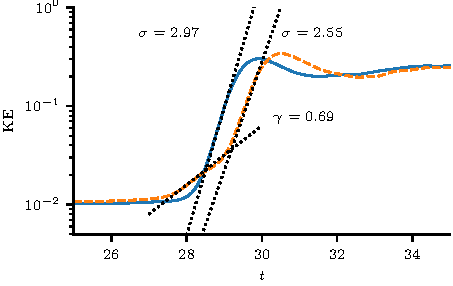
\includegraphics[width=\linewidth]{kinetic_energy_log-4.pdf}
      \caption{Growth rate estimation}
      \label{fig:kink_ke_log-4}
    \end{subfigure}
\caption{Kinetic energy as a function of time showing the development of the fluting and kink instabilities as well as their measured growth rates. Both plots are from results where $\eta=10^{-4}$.}
\label{fig:kink_str8_ke-4}%
\end{figure}

The onset of both the fluting and kink instabilities is seen in the kinetic energy profile only in the switching case (figure~\ref{fig:kink_ke_log-4}), where the nonlinear growth rates of the two instabilities are found to be $\gamma = 0.69$ for the fluting and $\sigma = 2.55$ for the kink. The onset times are approximately $t=27$ for the fluting instability and $t=28$ for the kink in both cases. In the isotropic case, the growth rate of the kink, $\sigma = 2.97$, is larger than in the switching case, and the kinetic energy profile shows no evidence of the growth of the fluting instability. By plotting the pressure directly (as is done later in figure~\ref{fig:pressure_pert_4}) it is found that a fluting perturbation is excited in the isotropic case, however its growth is damped by isotropic viscosity and the faster-growing kink instability quickly dominates. 

The faster growth of the kink compared to, say that of chapter~\ref{chp:kink_instability} is due to the relative aspect ratios of the flux tubes. The tube prescribed in~\ref{chp:kink_instability} has an aspect ratio of approximately $20$ compared to the tube studied here, which has an aspect ratio of approximately $4$. While the total twist is similar in both tubes (after the drivers have injected twist up to $t\approx20$) the small aspect ratio results in more turns per unit length, resulting in a more unstable instability.

%The slower kink growth rate in the switching case appears to be due to the fluting instability disrupting the linear kink perturbation and reducing its growth as a result. A similar effect is found in the simulations where $\eta=10^{-3}$.

\begin{figure}[t]
  \centering
    \begin{subfigure}{0.49\textwidth}
      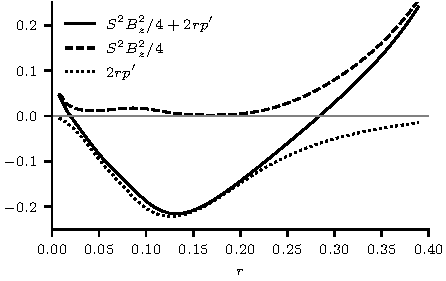
\includegraphics[width=\linewidth]{suydam_condition_4.pdf}
      \caption{Suydam condition}
      \label{fig:suydam_condition_4}
    \end{subfigure}
    \hfill
    \begin{subfigure}{0.49\textwidth}
      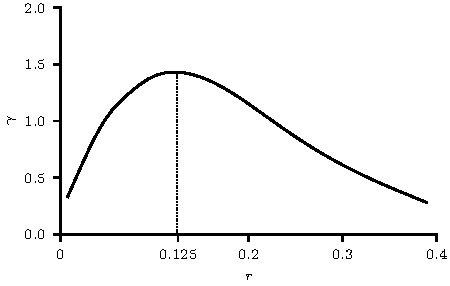
\includegraphics[width=\linewidth]{growth_rate_4.pdf}
      \caption{Linear growth rate}
      \label{fig:growth_rate_4}
    \end{subfigure}
\caption{Plots of Suydam's stability criterion and contributing terms (LHS of~\eqref{eq:suydams_criterion}) and predicted linear growth rate~\eqref{eq:fluting_growth_rate2} at $t=20$ for $\eta=10^{-4}$ and using the switching model. The location of the peak linear growth rate is also shown.}
\label{fig:stability_and_growth}%
\end{figure}

Prior to the onset of either instability, the flux tube is found to be linearly unstable to perturbations of the form~\ref{eq:kink_perturbation} at $t=20$ via Suydam's criterion~\ref{eq:suydams_criterion} (figure~\ref{fig:suydam_condition_4}). The criterion represents a balance between destabilising pressure gradients and stabilising magnetic shear. The shear is so small and the pressure gradient so large that the tube is unstable over a wide range of radii, from $r\approx 0.01$ to $0.3$. The measure of linear fluting growth rate $\gamma$ is plotted as a function of $r$ at the same time (figure~\ref{fig:growth_rate_4}). While the magnitude of the linear growth rate is not observed (and is difficult to observe in this setup regardless) the location of the peak growth well predicts the location of the resonant surface where the observed perturbation grows (figure~\ref{fig:swi-4_pressure_13}).

\begin{figure}[t]
  \centering
    \begin{subfigure}{0.49\textwidth}
      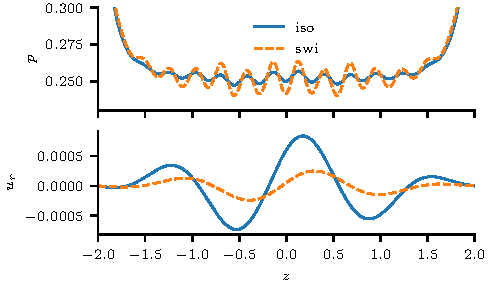
\includegraphics[width=\linewidth]{perturbations_4.pdf}
      \caption{Perturbations}
      \label{fig:pressure_pert_4}
    \end{subfigure}
    \hfill
    \begin{subfigure}{0.49\textwidth}
      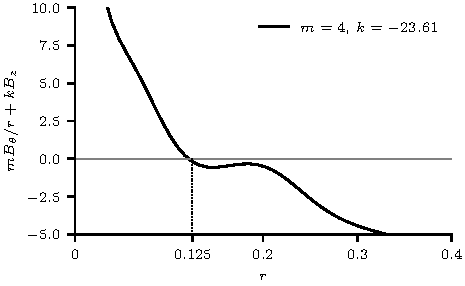
\includegraphics[width=\linewidth]{resonant_surface_4.pdf}
      \caption{Resonance function}
      \label{fig:resonant_surface_4}
    \end{subfigure}
\caption{Plots of the pressure and velocity perturbations in $z$ (corresponding to the fluting and kink instabilities, respectively) and of the resonance function $m B_{\theta}(r)/r + kB_z(r)$ as a function of $r$ using the observed fluting perturbation wavenumbers. All plots are from snapshots at $t=26$ where $\eta=10^{-4}$ and the viscosity model is switching.}
\label{fig:k_and_resonance}%
\end{figure}

Figure~\ref{fig:pressure_pert_4} plots the observed perturbations corresponding to the fluting and kink instabilities at $t=26$. The fluting perturbation is observed in the pressure and is plotted as a function of $z$ following a line through the point $(r, \theta) = (0.101, 0)$. The kink instability is observed in the $x$-velocity through the point $(x, y) = (0,0)$. Comparing the magnitudes of the perturbations suggests the fluting instability is nonlinear at this point while the kink instability likely remains linear.

The value of $k$ for each perturbation is calculated as $k = 2\pi/\tilde{\lambda}$ where $\tilde{\lambda}$ is the wavelength of the perturbation, measured as the difference between two of the peaks. This gives a value of $k_{flute}=23.61$ and $k_{kink}=4.57$ for both viscosity models. Hence, the observed most unstable fluting perturbation is that of the form~\ref{eq:kink_perturbation} where $m=4$ and $k=23.61$ and the observed kink instability is that where $m=1$ and $k=4.57$. Using these values, it is observed that the fluting perturbation resonates with the field, that is $m B_{\theta}(r)/r + kB_z(r) = 0$, at $r=0.125$ (figure~\ref{fig:resonant_surface_4}). This is precisely the predicted radius of peak linear growth (figure~\ref{fig:growth_rate_4}), although at this time the perturbation appears to approximately resonate over a range of radii from $r=0.125$ to $0.2$, likely an effect of the nonlinear development of the instability.

Comparing the effect of the viscous models on the perturbations, in the isotropic case, the fluting perturbation is damped, while in the switching case the kink perturbation is diminished, explaining why the fluting instability appears more readily in the switching case (figure~\ref{fig:kink_ke-4}).

\subsection{Development where $\eta=10^{-3}$}

\begin{figure}[t]
  \centering
    \begin{subfigure}{0.32\textwidth}
      \includegraphics[width=\linewidth]{swi-3_pressure_12.pdf}
      \caption{$t=24$}
      \label{fig:swi-3_pressure_12}
    \end{subfigure}
    \hfill
    \begin{subfigure}{0.32\textwidth}
      \includegraphics[width=\linewidth]{swi-3_pressure_14.pdf}
      \caption{$t=28$}
      \label{fig:swi-3_pressure_14}
    \end{subfigure}
    \hfill
    \begin{subfigure}{0.32\textwidth}
      \includegraphics[width=\linewidth]{swi-3_pressure_15.pdf}
      \caption{$t=30$}
      \label{fig:swi-3_pressure_15}
    \end{subfigure}
    \hfill
    \begin{subfigure}{0.32\textwidth}
      \includegraphics[width=\linewidth]{swi-3_pressure_16.pdf}
      \caption{$t=32$}
      \label{fig:swi-3_pressure_16}
    \end{subfigure}
    \hfill
    \begin{subfigure}{0.32\textwidth}
      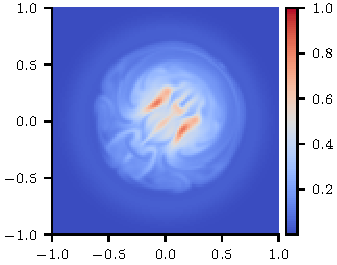
\includegraphics[width=\linewidth]{swi-3_pressure_17.pdf}
      \caption{$t=34$}
      \label{fig:swi-3_pressure_17}
    \end{subfigure}
    \hfill
    \begin{subfigure}{0.32\textwidth}
      \includegraphics[width=\linewidth]{swi-3_pressure_18.pdf}
      \caption{$t=36$}
      \label{fig:swi-3_pressure_18}
    \end{subfigure}
\caption{Pressure profiles through $z=0$ during the development of the fluting and kink instabilities. The viscosity model is switching and $\eta = 10^{-3}$. In contrast to the case of $\eta=10^{-4}$, the nonlinear development of the fluting instability has time to mix the interior of the flux tube before the onset of the kink instability, the growth of which is affected by the mixed plasma.}
\label{fig:kink_pressure_slices-3}%
\end{figure}

Figures~\ref{fig:kink_pressure_slices-3} show the prolonged development of the fluting instability and the slow nonlinear development of the kink. Due to the enhanced Ohmic heating when $\eta=10^{-3}$, the pressure gradient is substantially stronger than when $\eta=10^{-4}$ and the fluting instability is excited much earlier. Compared to the $\eta=10^{-4}$ cases, the instability occurs further from the axis, at $r\approx0.16$, and the larger pressure gradient drives the bulges further from the axis in the nonlinear phase (figure~\ref{fig:swi-3_pressure_12}). These bulges continue to extend outwards and mix the plasma in their wake. The kink instability can be observed moving the axis of the tube diagonally upwards and to the right in figure~\ref{fig:swi-3_pressure_15}. At this time in the $\eta=10^{-4}$ cases, the nonlinear development of the kink was further along (figure~\ref{fig:swi-4_pressure_15}). The development of the kink then proceeds slowly as it moves the axis of the tube through the mixed region to eventually begin the reconnection process with the outer region of field that is typical of the instability in this kind of flux tube (as was observed in chapter~\ref{chp:kink_instability}).

\begin{figure}[t]
  \centering
    \begin{subfigure}{0.49\textwidth}
      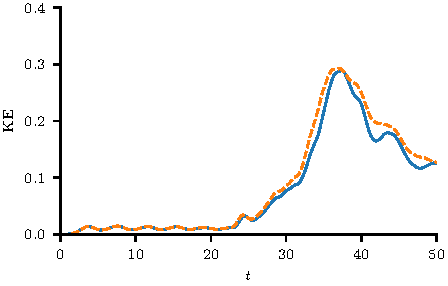
\includegraphics[width=\linewidth]{kinetic_energy-3.pdf}
      \caption{Kinetic Energy}
      \label{fig:kink_ke-3}
    \end{subfigure}
    \hfill
    \begin{subfigure}{0.49\textwidth}
      \includegraphics[width=\linewidth]{kinetic_energy_log-3.pdf}
      \caption{Growth rate estimation}
      \label{fig:kink_ke_log-3}
    \end{subfigure}
\caption{Kinetic energy as a function of time in the cases where $\eta=10^{-3}$. The results from both viscosity models are shown. The fluting instability appears earlier than where $\eta=10^{-4}$ and the growth rate of the kink instability is decreased.}
\label{fig:kink_str8_ke-3}%
\end{figure}

It is evident from the kinetic energy profile that the fluting instability develops much earlier than in the $\eta=10^{-4}$ cases and grows at an increased rate of $\gamma = 1.06$ (figure~\ref{fig:kink_ke_log-3}). As indicated earlier, the kink instability indeed grows at a slow rate of $\sigma \approx 0.15$, much lower than that observed in the $\eta=10^{-4}$ cases, and much lower than the earlier fluting instability. One key observation is that, despite the early and disruptive growth of the fluting instability, the kink instability still generates the bulk of the kinetic energy (figure~\ref{fig:kink_ke-3}).

Due to the influence of the drivers on the kinetic energy, the fluting growth rate is difficult to estimate from the kinetic energy profile as accurately as in the $\eta=10^{-4}$ cases. Since the kink instability occurs after the development of the fluting, its growth rate is similarly difficult to gauge. Nevertheless, it is clear that the fluting instability grows at a rate of the same order as that in the $\eta=10^{-4}$ case. It is also apparent that the kink instability grows much slower in the $\eta=10^{-3}$ case.

\begin{table}[]
\centering
\begin{tabular}{ccc}
&
$\eta=10^{-4}$ &
$\eta=10^{-3}$ \\
\midrule
%Predicted linear $\gamma$ & 1.43 & 2.72  \\
Observed nonlinear $\gamma$ & 0.69 & 1.06  \\
Observed $\sigma$ & 2.55 & 0.15\\
\midrule
Radius of peak $\gamma$ & 0.125 & 0.163 \\
Observed $r_s$ & 0.125 & 0.163 \\
\midrule
Observed $k_{flute}$ & 23.61 & 16.05 \\
Observed $k_{kink}$ & 4.57 & 4.53 \\
\end{tabular}
\caption{Quantitative differences in the observed perturbations between results for both values of $\eta$. See text for details of measurements times.}
\label{tab:kink_fluting_params}
\end{table}

Table~\ref{tab:kink_fluting_params} summarises the quantitative differences between the results using the two values of $\eta$. All values are calculated from simulations using the switching model due to the similarity with the switching results with the exception of $k_{kink}$ which is measured from isotropic results due to noise in the switching case. The radius of peak $\gamma$ is calculated at time $t=20$. The fluting wavenumber $k$ and observed $r_s$ are measured at times just prior to the nonlinear development of the fluting instability, that is at $t=22$ when $\eta=10^{-3}$ and $t=26$ when $\eta = 10^{-4}$. The kink wavenumber is measured at $t=26$ in both cases. These times allow fair comparison between measurements.

The longitudinal wavenumber $k_{kink}$ of the observed kink perturbation remains similar in both cases since the instability is essentially governed by the twist injected by the driver which remains the same in both cases. In contrast, the longitudinal wavenumber $k_{flute}$ of the observed fluting perturbation is lower in the $\eta=10^{-3}$ cases. This is due to the different resonant surface within which the perturbation grows, as dictated by the peak of the linear growth rate. We note that this peak again matches well the location of the observed resonant surface, as in the $\eta=10^{-4}$ cases.

\section{Discussion}

Due to the perturbations arising from numerical noise, it is likely that the $m=4$ perturbation is excited due to influences from the boundaries in the Cartesian box, for example through the interaction of reflected fast waves. Performing a similar experiment in a cylindrical numerical domain, or imposing a variety of perturbations in the Cartesian domain may reveal other, faster growing modes. The modes may also be influenced by nonlinear coupling between the $m>1$ and $m=1$ modes, as is found in the study of kink and fluting oscillations.

It is known that the fluting mode in oscillating flux tubes can be generated through nonlinear coupling to the large-scale kink mode~\cite{terradasEffectMagneticTwist2018,rudermanNonlinearGenerationFluting2017a}. It may be that the fluting and kink instabilities are similarly able to couple and influence one another. Certainly, we have found in this set of experiments that the mixing as a result of the nonlinear fluting instability appears to slow the growth of the kink instability. In the linear regime it seems unlikely that the linear perturbations of either the fluting or kink would be able to interact, given that the kink instability generally presents at the axis of a flux tube and the fluting at some resonant surface away from the axis. Further investigate of the nonlinear interaction between the two instabilities is required.

Since the main driver of the fluting instability is the pressure gradient generated through Ohmic heating, it is prudent to ask if the same pressure gradient could be generated using physical coronal values of the resistivity (of approximately $\eta=10^{-8}$~\cite{craigAnisotropicViscousDissipation2009a}) which are much smaller than those studied here. We note that Ohmic heating scales with $\eta j^2$ and not necessarily with $\eta$ itself so, even at realistic values of $\eta$, Ohmic heating may be sufficient to generate gradients unstable to the fluting instability in real coronal loops, given a strong enough current density. Running a similar experiment with realistic values of the resistivity is currently computationally infeasible, so direct experimentation is unavailable.

What is suggested by our results is that a flux tube can be unstable to the fluting instability and yet the faster growing kink instability can quickly dominate when the pressure gradient is small enough that the fluting instability grows slower than the kink. However, we also find the opposite case, where the faster growing fluting instability appears to slow the growth of the kink instability although, importantly, it does not fully disrupt the development of the kink. Understanding the balance between the nonlinear growth rates of the two instabilities is important in understanding whether the fluting instability may be found at all in the real solar corona, or whether its realistic growth rate is simply too slow compared to that of the kink instability.

Regardless of the heating mechanism, coronal loops with strong radial pressure gradients have been observed~\cite{foukalTemperatureStructurePressure1975}. Such loops may be unstable to the fluting instability so it would be instructive to investigate these using a similar numerical experiment to that performed in chapter~\ref{chp:kink_instability}, though with a kink-stable loop. Alternatively, observations may reveal loops which have already undergone internal fluting instabilities to stabilise a pressure gradient. Forward modelling of a loop where the fluting instability has been excited (but not the kink) would provide a useful comparison to observations.

\section{Conclusion}

This chapter details the nonlinear development of two ideal instabilities, the kink and fluting instabilities, both of which develop naturally in the course of twisting an initially straight magnetic flux tube. This provides a different approach to the simulations performed in chapter~\ref{chp:kink_instability} in that the instabilities are not excited by any prescribed perturbations and the field is dynamically driven into an unstable state. Not only is the kink instability excited directly due to the twist in the field, we find a pressure-driven fluting instability is also excited by pressure gradients generated by Ohmic heating.

We find that the fluting instability can be quickly dominated by the kink instability if the kink grows substantially faster than the fluting. However, if the fluting has time to develop nonlinearly, it mixes the plasma within the flux tube, generating small scale current sheets and releasing some magnetic potential energy. The overall effect of this mixing is to slow the growth of the kink instability. The slowed growth of the kink does not appear to impact the total energy release, only the time over which it is released. 

These numerical experiments have provided evidence that the fluting instability can occur in twisted magnetic flux ropes and grow at similar rates to the kink instability. However, this provides a proof-of-concept at best. Further investigation of the relative growth rates in more realistic coronal loop setups is required to fully understand if the fluting instability plays a pertinent role in coronal loop physics.
